\documentclass{article}\usepackage{graphicx, color}
%% maxwidth is the original width if it is less than linewidth
%% otherwise use linewidth (to make sure the graphics do not exceed the margin)
\makeatletter
\def\maxwidth{ %
  \ifdim\Gin@nat@width>\linewidth
    \linewidth
  \else
    \Gin@nat@width
  \fi
}
\makeatother

\IfFileExists{upquote.sty}{\usepackage{upquote}}{}
\definecolor{fgcolor}{rgb}{0.2, 0.2, 0.2}
\newcommand{\hlnumber}[1]{\textcolor[rgb]{0,0,0}{#1}}%
\newcommand{\hlfunctioncall}[1]{\textcolor[rgb]{0.501960784313725,0,0.329411764705882}{\textbf{#1}}}%
\newcommand{\hlstring}[1]{\textcolor[rgb]{0.6,0.6,1}{#1}}%
\newcommand{\hlkeyword}[1]{\textcolor[rgb]{0,0,0}{\textbf{#1}}}%
\newcommand{\hlargument}[1]{\textcolor[rgb]{0.690196078431373,0.250980392156863,0.0196078431372549}{#1}}%
\newcommand{\hlcomment}[1]{\textcolor[rgb]{0.180392156862745,0.6,0.341176470588235}{#1}}%
\newcommand{\hlroxygencomment}[1]{\textcolor[rgb]{0.43921568627451,0.47843137254902,0.701960784313725}{#1}}%
\newcommand{\hlformalargs}[1]{\textcolor[rgb]{0.690196078431373,0.250980392156863,0.0196078431372549}{#1}}%
\newcommand{\hleqformalargs}[1]{\textcolor[rgb]{0.690196078431373,0.250980392156863,0.0196078431372549}{#1}}%
\newcommand{\hlassignement}[1]{\textcolor[rgb]{0,0,0}{\textbf{#1}}}%
\newcommand{\hlpackage}[1]{\textcolor[rgb]{0.588235294117647,0.709803921568627,0.145098039215686}{#1}}%
\newcommand{\hlslot}[1]{\textit{#1}}%
\newcommand{\hlsymbol}[1]{\textcolor[rgb]{0,0,0}{#1}}%
\newcommand{\hlprompt}[1]{\textcolor[rgb]{0.2,0.2,0.2}{#1}}%

\usepackage{framed}
\makeatletter
\newenvironment{kframe}{%
 \def\at@end@of@kframe{}%
 \ifinner\ifhmode%
  \def\at@end@of@kframe{\end{minipage}}%
  \begin{minipage}{\columnwidth}%
 \fi\fi%
 \def\FrameCommand##1{\hskip\@totalleftmargin \hskip-\fboxsep
 \colorbox{shadecolor}{##1}\hskip-\fboxsep
     % There is no \\@totalrightmargin, so:
     \hskip-\linewidth \hskip-\@totalleftmargin \hskip\columnwidth}%
 \MakeFramed {\advance\hsize-\width
   \@totalleftmargin\z@ \linewidth\hsize
   \@setminipage}}%
 {\par\unskip\endMakeFramed%
 \at@end@of@kframe}
\makeatother

\definecolor{shadecolor}{rgb}{.97, .97, .97}
\definecolor{messagecolor}{rgb}{0, 0, 0}
\definecolor{warningcolor}{rgb}{1, 0, 1}
\definecolor{errorcolor}{rgb}{1, 0, 0}
\newenvironment{knitrout}{}{} % an empty environment to be redefined in TeX

\usepackage{alltt}
\usepackage{times}
\usepackage{ie07}
\usepackage{hyperref}
\usepackage{amsmath}

% put paranthesis after equation
% http://www.latex-community.org/forum/viewtopic.php?f=4&t=334
\makeatletter
\def\tagform@#1{\maketag@@@{\ignorespaces#1\unskip\@@italiccorr}}
\let\orgtheequation\theequation
\def\theequation{(\orgtheequation)}
\makeatother
    




\begin{document}


\title{AN OPEN SOURCE TOOL TO ESTIMATE MASS AND EFFICIENCY OF WIND TURBINE POWER TAKE-OFF SYSTEMS}

\authorname{Ozan Keysan, Markus A. Mueller}
\authoraddr{Institute for Energy Systems, University of Edinburgh, EH93JL, U.K.\\
Email: o.keysan@ed.ac.uk}

\maketitle

\keywords
Wind turbine, mass estimation, direct-drive, gearbox, generator

\abstract
This is where the abstract should be placed. It should
consist of one paragraph and a concise summary of the
material discussed in the article below. It is preferable not
to use footnotes in the abstract or the title. The
acknowledgement for funding organisations etc. is placed
in a separate section at the end of the text. We wish you
success with the preparation of your manuscript.

\section{Introduction}

Far offshore wind turbines can help to exploit the wind energy resources that remained untapped so far. These turbines are planned to be installed as floating platforms due to  high water depths (\textgreater 40 m). Reliability and mechanical stability is the most important issues of floating wind turbines. The nacelle mass is critical for the mechanical stability of the platform \cite{Sethuraman2013,Christiansen2011}. A higher mass on the top of the tower increases the center of mass significantly, and this should be balanced with a larger ballast, which increases the installation cost. 

Although, doubly-fed induction generator coupled to a multi-stage gearbox is the most common power take-off (PTO) type for onshore wind turbines; it may not be the most suitable option for a large offshore wind turbine. A direct-drive power take-off systems can be used to eliminate the gearbox, but the mass of a direct-drive generator can be larger than a high-speed power take-off system depending on the power rating and diameter.

In this study, data from manufacturers and literature are collected to predict the  mass and efficiency trend lines for wind turbine components. These equations are used to build an open-source tool that can estimate the mass and efficiency of the total power take-off system. Users can modify the data and models using the tools defined in Appendix-A.

\section{Power Take-Off Components}

The main power take-off components in a wind turbine can be listed as: bearing, shaft, gearbox (if applicable), and generator. 

\subsection{Gearbox}

\subsubsection{Multi Stage Gearbox}

The most common gearbox type used in wind turbines is the three-stage gearboxes, which increase the turbine speed to approximately 1500 rpm. 
Data from the following three-stage wind turbine gearbox manufacturers are collected: Bosch-Rexroth\cite{bosch}, Winergy\cite{winergy}, Moventas\cite{Moventas}, Eickhoff\cite{eickhoff}, and General Electric\cite{GE}, and plotted in \autoref{fig:gearbox}. From the figure, it may be seen that the mass of the gearbox is proportional to input torque, which is represented as a linear function in \autoref{3G_gearbox}. 

\begin{knitrout}
\definecolor{shadecolor}{rgb}{0.969, 0.969, 0.969}\color{fgcolor}\begin{figure}[]

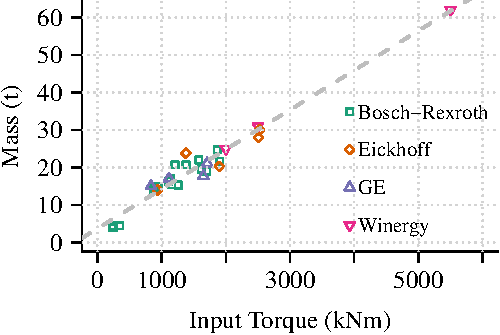
\includegraphics[width=\maxwidth]{figure/gearbox} \caption[Mass of three-stage gearboxes versus torque]{Mass of three-stage gearboxes versus torque.\label{fig:gearbox}}
\end{figure}


\end{knitrout}


\begin{equation}
\text{Mass(t)} = 0.011 \times T_{in} + 3.7
\label{3G_gearbox}
\end{equation}


Multi-stage gearboxes usually consist of two planetary gear stages and an additional high-speed parallel-shaft helical gear stage. In \cite{Hau2005a} it is stated that each planetary gear stages have 1 \% power loss and each helical gear stages have 2 \% power loss. Thus, the efficiency of a three-stage gearbox can be represented as in \autoref{3G_efficiency} \cite{Zhang2011a}. The equation implies that the efficiency of a three-stage gearbox varies from 97 \% at no load to 96 \% at full load.

\begin{equation}
  \text{Efficiency(\%)} = 97.0 - \dfrac{P_{in}}{P_{rated}}
  \label{3G_efficiency}
\end{equation}

\subsubsection{Single Stage Gearbox}

Gear ratios up to 15:1 can be achieved using a single stage gearbox \cite{Cotrell2002}. Single-stage gearboxes usually consist of a planetary stage with various numbers of gears depending on the power rating. Single stage gearboxes have fewer gears and bearings than high-speed gearboxes, which inreases the reliability. Moreover, their efficiencies are higher than multi-stage gearboxes. In \cite{Matveev2011}, the efficiency of a single stage gearbox is given as:

\begin{equation}
  \text{Efficiency(\%)} = 99.5 - \dfrac{P_{in}}{P_{rated}}
\end{equation}

Mass of a single-stage gearbox coupled with medium-speed generator can be approximated as in \cite{Fingersh2006}:

\begin{equation}
	\text{Mass(t)} = 88.3 \times {T_{in(kNm)}}^{0.774}
\end{equation}

where $T_{input}$ is the input torque in kNm.


\subsection{Structural Components}

\subsubsection{Low Speed Shaft}
Low speed shaft is not a critical component; it connects the main hub to the gearbox or to the generator. Low speed shaft is not required for some drive train options (e.g. integrated bearing type). In \cite{Fingersh2006}, the mass and the cost of the low speed shaft is presented as a function of the turbine diameter.

\begin{equation}
		\text{Mass (t)} = 1.35 \times {P_{rated(MW)}}^{1.44}
\end{equation}

\subsubsection{Main Bearing}

The mass of the main bearing can vary depending on the bearing type. For example, a double-tapered roller bearing for a direct-drive is heavier than a conventional two-point suspension type bearing. In  \cite{Fingersh2006}, the mass of the main bearing is presented as a function of turbine diameter. Assuming mass of the bearing housing is equal to bearing mass, the mass of the main bearing system can be expressed as a function of the rated power as in \autoref{mass_bearing}.

\begin{equation}
	\text{Mass(t)} = 0.26 \times {P_{rated(MW)}}^{1.75}
  \label{mass_bearing}
\end{equation}

\subsection{Hydraulic Systems}

\subsection{Generator}

The generator types covered are induction generator, permanent-magnet generator, synchronous generator and superconducting generator. The cooling methods for induction and synchronous generators are also defined (air-cooled or water-cooled). 

\subsubsection{Induction Generator}

Induction generators are the most common generator type used in wind turbines. Squirrel cage induction generators are preffered for small wind turbines, where doubly-fed induction generators are preffered for large wind turbines. Mass data for various power rated machines (4-poles) from ABB and Siemens catalogues are collected \cite{ABB2012, Siemens}, which are plotted in \autoref{fig:induction_generator}. Trend lines for Siemens machines show that, the water-cooled induction generators are 18 \% lighter than the air-cooled ones. The mass of generators as a function of the rated power can be expressed as in \autoref{mass-air} and \autoref{mass-water}.

Efficiencies of induction generators at rated load are plotted in \autoref{fig:induction_generator_efficiency}. The efficiency does not change with the cooling method, but increases with the power rating (efficiency increases from 96 \% to 97.5 \% as the power rating is increased from 2 MW to 8 MW). 

\begin{equation}
  \text{Mass}_{air-cooled}(t) = 3.91 \times {P_{rated(MW)}}^{0.69}
  \label{mass-air}
\end{equation}

\begin{equation}
  \text{Mass}_{water-cooled}(t) = 3.22 \times {P_{rated(MW)}}^{0.68}
  \label{mass-water}
\end{equation}

\begin{equation}
\text{Efficiency (\%)} = 95.64 \times {P_{rated(MW)}}^{0.01}
\end{equation}


\begin{knitrout}
\definecolor{shadecolor}{rgb}{0.969, 0.969, 0.969}\color{fgcolor}\begin{figure}[]

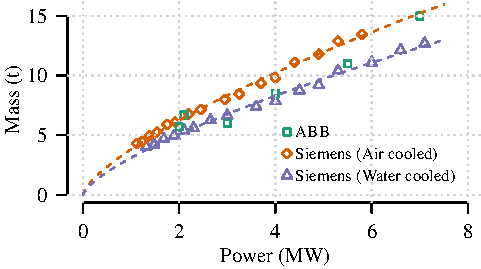
\includegraphics[width=\maxwidth]{figure/induction_generator} \caption[Mass of the induction generator vs torque]{Mass of the induction generator vs torque.\label{fig:induction_generator}}
\end{figure}


\end{knitrout}


\begin{knitrout}
\definecolor{shadecolor}{rgb}{0.969, 0.969, 0.969}\color{fgcolor}\begin{figure}[]

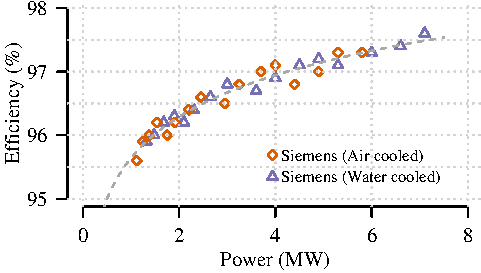
\includegraphics[width=\maxwidth]{figure/induction_generator_efficiency} \caption[Efficiency of induction generator at rated load vs power rating]{Efficiency of induction generator at rated load vs power rating.\label{fig:induction_generator_efficiency}}
\end{figure}


\end{knitrout}



\subsubsection{Direct-Drive Synchronous Generator}

Electrically excited direct-drive synchronous generators can be used in wind turbines to reduce the raw material cost compared to direct-drive permanent magnet generators. One example is the 7.5 MW, 13 rpm Enercon 126 wind turbine, with a generator mass of 220 t.
In \cite{upwind2011}, various direct-drive synchronous generator designs are presented from 0.75 MW to 10 MW. It is better to calculate the mass of direct-drive generators as a function of the input torque, since the rotational speed changes with power rating. The linear equation that represents the mass of a direct-drive synchronous generator is given in \autoref{eesg_mass}.

\begin{equation}
  \text{Mass(t)} = 0.035 \times {T_{rated(kNm)}} + 8.9
  \label{eesg_mass}
\end{equation}

\subsubsection{Direct-Drive Permanent Magnet Generator}

Direct-drive permanent magnet generators have higher torque densities than electrically excited synchronous machines. Some notable direct-drive permanent magnet generators are: Harakosan (1.5 MW, 18 rpm, 47.2 t), The Switch (3.8 MW, 21 rpm, 81 t) \cite{Duan2009}. In \cite{Bang2008,upwind2011} many other permanent-magnet designs are presented. There are a few other designs to reduce the mass of PM machines, transverse-flux machine is being one of them as presented in \cite{Bang2009}. However, radial flux permanent magnet machine is the most common topology, and therefore it is used for mass estimation as presented in \autoref{mass_ddpm}.

\begin{equation}
  \text{Mass(t)} = 0.028 \times {T_{rated}} + 2.8
  \label{mass_ddpm}
\end{equation}


\subsubsection{Medium Speed Permanent Magnet Generator}

\begin{equation}
  \text{Mass(t)} = 0.03 \times {T_{rated}} + 1.5
\end{equation}

As shown in \autoref{fig:plot1gpm}

\begin{knitrout}
\definecolor{shadecolor}{rgb}{0.969, 0.969, 0.969}\color{fgcolor}\begin{figure}[]

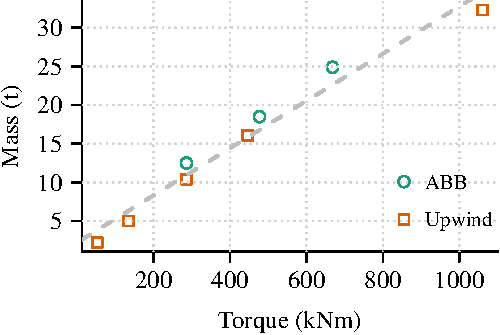
\includegraphics[width=\maxwidth]{figure/plot1gpm} \caption[Mass of the medium speed permanent magnet generator vs torque]{Mass of the medium speed permanent magnet generator vs torque.\label{fig:plot1gpm}}
\end{figure}


\end{knitrout}



\section{Open Source Tool}
All these data are combined in an open-source design tool. The user can select different PTO systems, and then define the input power and rotational speed The design tool gives the mass and efficiency of the components. Thus, it is very easy for a user to compare different PTO systems and modify the mechanical models based on these estimations. The design tool is built using Matlab GUI. The aim of the study is to publish it as a web application that is open to wind turbine designers. We aim to expand the toolbox for the reliability calculation of the different PTO systems. The design tool will help the designers to compare different PTO systems and select the most suitable option for the specific application.

\section*{Acknowledgements}
The acknowledgement for funding organisations etc.
should be placed in a separate section at the end of the
text. Thank you for your cooperation in complying with
these instructions.

\bibliography{IET_RPG_2013}
\noindent
\bibliographystyle{plain}

\end{document}
